\documentclass{article}
\usepackage[T1]{fontenc}
\usepackage{lmodern}
\usepackage{graphicx}
\usepackage{amsmath,amssymb}
\usepackage[a4paper,margin=2cm]{geometry}
\usepackage[absolute,overlay]{textpos}
\setlength{\TPHorizModule}{1mm}
\setlength{\TPVertModule}{1mm}
\usepackage[indonesian]{babel}
\usepackage{hyperref}
\setlength{\emergencystretch}{2em}
% unit: Halaman 102

\begin{document}

% === Halaman 102 (llm) ===

\begin{itemize}
    \item Untuk matriks $3 \times 3$, matriks dapat dicari dengan metode Eliminasi Gauss-Jordan, atau dihitung langsung dengan rumus berikut::
\end{itemize}

\vspace{10mm}

\begin{itemize}
    \item yang dalam hal ini,
\end{itemize}

\begin{align*}
 A &= (ei - hf) & B &= -(di - fg) & C &= (dh - eg) \\
 D &= -(bi - hc) & E &= (ai - cg) & F &= -(ah - bg) \\
 G &= (bf - ec) & H &= -(af - cd) & I &= (ae - bd)
\end{align*}

dan

\[ 
\det(\mathbf{K}) = aA + bB + cC
\]

% deskripsi: Rumus perhitungan invers matriks 3x3 menggunakan determinan dan matriks kofaktor yang ditranspose.
% bbox normalisasi: [0.1800, 0.2300, 0.7700, 0.3900]
\begin{textblock*}{123.90mm}(37.80mm,68.31mm)
\noindent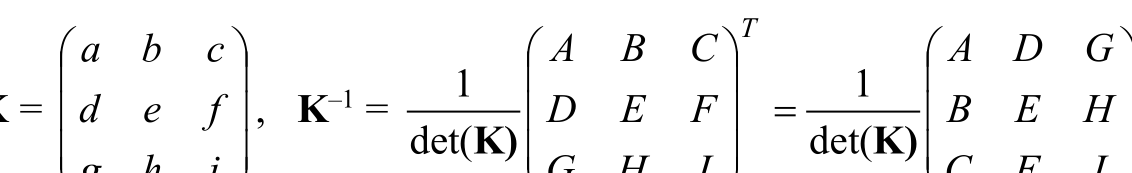
\includegraphics[width=123.90mm,height=47.52mm]{../../images/llm/page_102_img_01.png}%
\end{textblock*}

\end{document}
